% this is a template for an ``article'' document, the most common
% for research papers. Theses may be better written in the ``report''
% format.

% rename this file to foo.tex and then compile using 
%
%  latex foo
%
% view it with 
%
%  xdvi foo
%
% In order to print, create a PostScript file with
%
%  dvips foo
%
% then use
%
%  lpr -Pps2 foo.ps
%
% Have fun!
%
% Andreas
%
\documentclass{article}
\usepackage{amsmath}
\usepackage{paralist}

% set margins to 1 inch all around the page, no header or footer.
\setlength{\textheight}{9in}
\setlength{\textwidth}{6.5in}
\setlength{\topmargin}{-0.125in}
\setlength{\oddsidemargin}{-.2in}
\setlength{\evensidemargin}{-.2in}
\setlength{\headsep}{0in}

% enable insertion of graphics, ``smart'' line spacing, long tables
% for the long (i.e. more than 1 page) tables, refer to supertab.ps
\usepackage{setspace,supertabular}	

\usepackage[dvips]{graphicx}
% use \usepackage[dvips,draft]{graphicx} during document creation if
% you have screenshots in your file.


% output the list of used files to the terminal during compilation.
% this helps to keep track of the figures and tex-files you are using.
\listfiles

% set the path for figures.
% all figures should be in a subdirectory under the document directory
\graphicspath{{figures/}}

% define the line spacing. Footnotes and Caption remain single-spaced
\singlespacing
% alternatives: \onehalfspacing or \doublespacing or \setstretch{1.6}


% this was the preamble, now comes the main text
\begin{document}

\section{Robust Dynamic Programming}
Model based optimal control is a powerful tool but relies heavily on the accuracy of the system model, which is not a trivial task to derive. There are many parameters involved, such as friction, sensor readings, calibrations, and the model may change over time due to wear, temperature, humidity, contact condition, and others.

Eric Whitman looks into using Multiple Model Dynamic (MMD) Programming, and uses the inverted pendulum swing-up problem to demonstrate the algorithm.

 http://www.contrib.andrew.cmu.edu/~ewhitman/thesis.pdf

 
  By using the content provided in his thesis, the references, and example code, work on providing other students comprehensive guild on MMD for future students, we are looking at the different advantages, and shortcomings that comes with the algorithm.

Based on his previous work this paper aims to clarify the fundamental concepts of MMD and provide graspable examples. Furthermore, a faster running-time implementation using a General Purpose Graphical Processing Unit (GPGPU).

\subsection{Looking at a Problem}
	To have a better understanding on how the algorithm works, we are going to look at the  inverse pendulum swing-up example, which consists of a motor attached to the end of pendulum, and the controller aims to bring the pendulum to an upright position by applying torques based on the current state of the system. 

The expected behavior for the control law is to apply a torque equal to the direction the pendulum is swinging, such that more energy is added to the pendulum with each period, and when the pendulum finally has enough energy to perform a full rotation, apply a torque opposite to the movement such that the pendulum stops in an upright position.  

Since our interested is in solving a variety of dynamic programming problems, we are going to look at a more generic solution that discretizes the whole state of problem, and attempts to find a adequate policy to reach the desired goal.  

\pagebreak

\section{DARPA Robotics Challenge}
\paragraph{The objective of this paper is to help the reader understand the current workings of the Carnegie Mellon’s University’s controller.}  
 
The DARPA Robotics Challenge (DRC) is a competition of teams developing robots capable of assisting humans in responding to natural and man-made disasters.   
 
Teams are spread in several tracks. WPI is in the Track C team, in which competed in the Virtual Challenge (DVC), and received funding for the Atlas robot.  

\section{Hardware}
\subsection{Atlas}

The Atlas robot is a powerful robot in the form of an adult human. It is powered by 28 hydraulically-actuated rotation joints, with a closed-loop position and force control. It also contains a real time control computer (What is the specs?). Currently powered by external electricity, and packed with a head-mounted sensor package with LIDAR and stereo cameras. 

The robot gives the option of interchanging the hands, the two primary options being the iRobot© hands, and the Sandia© hands. While both options are known companies in the industry, neither provided the power, nor robustness necessary to complete the industrial tasks. These hands were designed to perform precision tasks, such as picking up a coin, or a fist-sized rock, but not to pick up a power tool. The team went to an alternative in using hardware developed Robotiq©, a 3-Finger adaptive robot gripper, which provided a much stronger grip. 

\subsection{DBI Behaviors}
Boston Dynamics provided predefined behaviour for Atlas, each of these controllers can be activated from state to another state. 

\subsubsection{Manipulate}
The Manipulation mode, in which the user can control all the joints above the torso, and basic control of the pelvis orientation, and the pelvis height. The legs are controlled by the Boston Dynamics controller embedded in the firmware.

It is fairly easy to use, and has a wide range of motion if the pelvis position and orientation is controlled together with an inverse kinematics solver for the joints, but can be unpredictable. The robot has the problem that the back joint that helps torso move back and forth is not strong enough to hold, and may give out a times, causing the whole top part of the robot fall forward, or at times, make the entire robot fall forward. 

The user has the option to input any additional weight that the hand is carrying to help the controller.

MoveIt! is a software developed with ROS to help robot developers control the robot. It contains a inverse kinematics solver that can interface with Atlas, but prevents two containing limitations: 
\begin{inparaenum}[\itshape a\upshape)]
\item The inverse kinematics solver has no option to give approximate solutions, and will fail to give joint state values unless a very approximate solution for a desired hand position exists.
\item It does not account for modifying the pelvis position and orientation for solving for a solution. \end{inparaenum}
 

\subsubsection{Walk}
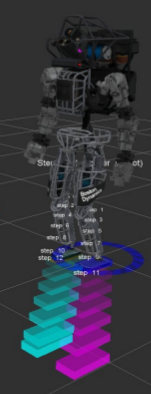
\includegraphics[width=2.5cm]{images/step_gui.png}

Boston Dynamics walking behaviour works by the user providing a sequence of steps paramters, which include the step duration, sway duration, swing height, lift height, and step end distance.  




\subsubsection{Atlas Control Parameters}
There exists several controller parameters that is hidden to the developer that controls the hydraulic joints. We let $q$, $qd$ and $f$ be the senses position, velocity, and torque respectively. And we let $q_d$, $qd_d$, and $f_d$ be the desired position, velocity, and torque for each joint.

We create the following variables to help control the desired torque control:

\begin{itemize}
\item $k_{q_p}$: Position error gain, in $\frac{N \cdot m}{rad}$.
\item $k_{q_i} $: Integral of position error gain, in $\frac{N \cdot m}{rad \cdot s}$.
\item $k_{{qd}_p}$: Derivative error gain, in $\frac{N \cdot m}{\frac{rad}{s}}$.
\item $k_{f_p}$: Proportional force feedback gain.
\item ${ff}_{qd}$: Feedforward velocity gain.
\item ${ff}_{{qd}_d}$: Feedforward desired velocity gain.
\item ${ff}_{f_d}$: Feedforward desired force gain.
\item ${ff}_{const}$: Constant force term.
\end{itemize}

And use them accordingly: 
\begin{align*}
k_{q_p} &\cdot ( q_d - q ) &+\\
k_{q_i} &\cdot 1/s * ( q_d - q ) &+\\
k_{{qd}_p} &\cdot ( {qd}_d - qd ) &+\\
k_{f_p} &\cdot ( f_d - f ) &+\\
{ff}_{qd} &\cdot qd &+\\
{ff}_{{qd}_d} &\cdot qd_d &+\\
{ff}_{f_d} &\cdot f_d &+ {ff}_{const}
\end{align*}


\subsection{Robotiq Hand}

\section{Software}
\subsection{Architecture}
\subsection{Network}
\subsection{ROS}

\section{Full-body controller}
Intro...Carnegie Mellon University developed custom software for controlling the robot, which involves two major aspects that are solve using Quadratic programming, an Inverse Kinematics solver, and an Inverse Dynamics solver. 
\subsection{Inverse Kinematics}

\subsection{Inverse Dynamics}

\subsection{Quadratic Programming}

\subsection{Results}

\subsection{Conclusion}

\subsection{Future Work}

\section{DRC Valve}
\subsection{Approach}
\subsection{Results}
\subsection{Conclusion and Future Work}

\section{DRC Wall}
\subsection{Approach}
\subsection{Results}
\subsection{Conclusion and Future Work}

\section{Conclusion}

\section{Acknowledgment}




%write your main text here
%\LaTeX template.



%this is an example how to include a figure in eps-format. Refer to 
%latexguide.ps for more help.
% this example loads the file /figures/mychart.eps

%\begin{figure}[htb]
%  \begin{center}
%    \includegraphics[width=5cm]{mychart.eps}
%    \caption{A picture in \LaTeX}
%    \label{fig:my_first_figure}
%  \end{center}
%\end{figure}

\end{document}







